% sos2cayley evenblocks.sos --rename a=a,!a=b
% Generated by sosl.sos.viz. Every visual choice is in the \tikzset below:
% edit a style to restyle, edit a coordinate to move a node.
\documentclass[tikz,border=4pt]{standalone}
\usetikzlibrary{arrows.meta,shapes.misc}
\begin{document}
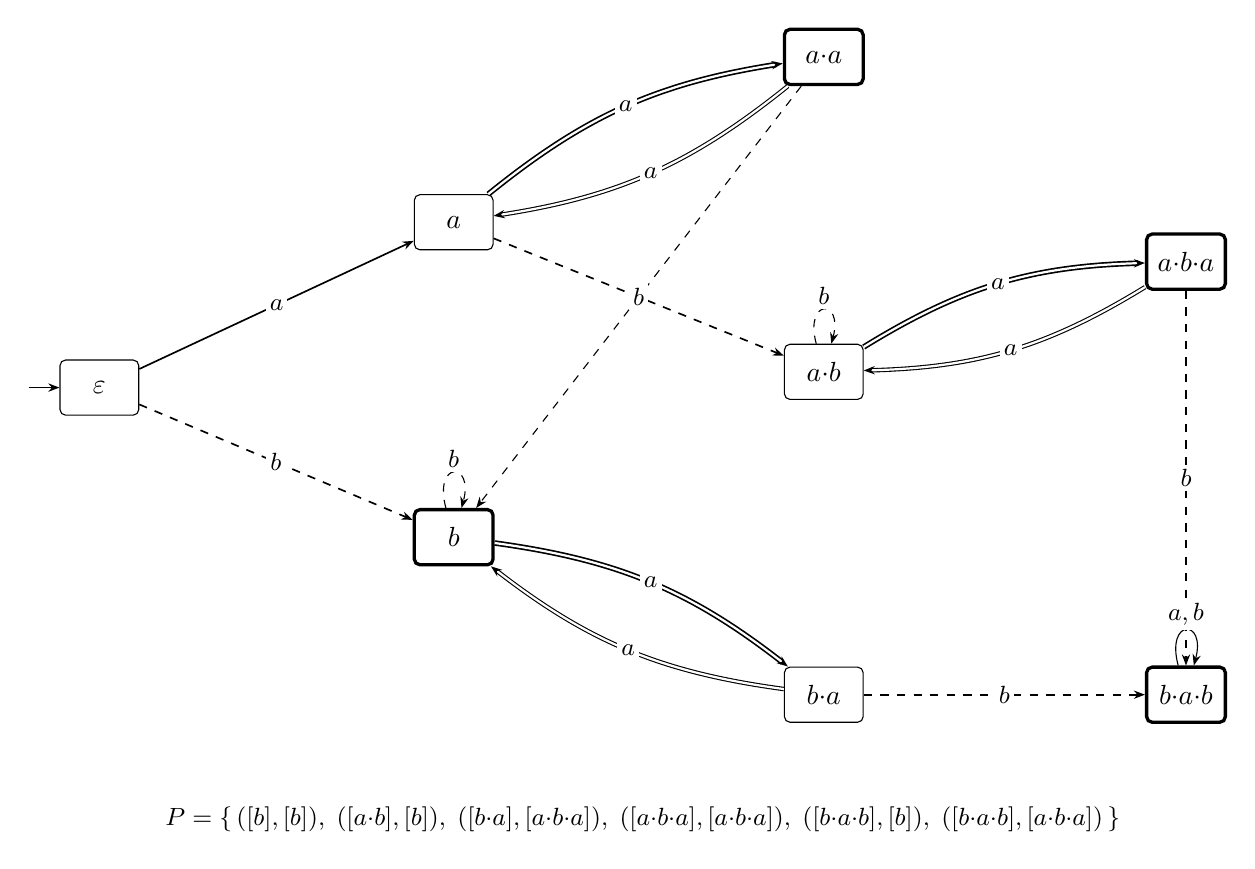
\begin{tikzpicture}[
  class/.style     = {draw, thin, rounded corners=2pt, inner sep=3pt,
                      minimum width=10mm, minimum height=7mm},
  root/.style      = {},          % the root needs no ink: the init stub says it
  idem/.style      = {very thick},
  init/.style      = {semithick, -{Stealth[length=4pt,width=3pt]}},
  letter a/.style = {solid},          % display letter a
  letter b/.style = {dashed},          % display letter b
  mixed/.style     = {solid},     % one arrow, several letters agree on it
  tree/.style      = {semithick, -{Stealth[length=4pt,width=3pt]}},
  nontree/.style   = {thin, -{Stealth[length=4pt,width=3pt]}},
  cyc/.style       = {double, double distance=0.8pt},
  lbl/.style       = {font=\small, inner sep=1.5pt, fill=white},
  pairs/.style     = {anchor=north, font=\small},
]

  \node[class,root] (eps) at (3.3,4.7) {$\varepsilon$};
  \node[class] (a) at (7.8,6.8) {$a$};
  \node[class,idem] (b) at (7.8,2.8) {$b$};
  \node[class,idem] (aa) at (12.5,8.9) {$a{\cdot}a$};
  \node[class] (ab) at (12.5,4.9) {$a{\cdot}b$};
  \node[class] (ba) at (12.5,0.8) {$b{\cdot}a$};
  \node[class,idem] (aba) at (17.1,6.3) {$a{\cdot}b{\cdot}a$};
  \node[class,idem] (bab) at (17.1,0.8) {$b{\cdot}a{\cdot}b$};

  % the root is the adjoined identity: a source, marked like an initial state
  \draw[init] (2.4,4.7) -- (eps);

  \draw[letter a,tree] (eps) to node[lbl] {$a$} (a);
  \draw[letter b,tree] (eps) to node[lbl] {$b$} (b);
  \draw[letter a,tree,cyc] (a) to[bend left=15] node[lbl] {$a$} (aa);
  \draw[letter b,tree] (a) to node[lbl] {$b$} (ab);
  \draw[letter a,tree,cyc] (b) to[bend left=15] node[lbl] {$a$} (ba);
  \draw[letter b,nontree] (b) to[loop above] node[lbl] {$b$} (b);
  \draw[letter a,nontree,cyc] (aa) to[bend left=15] node[lbl] {$a$} (a);
  \draw[letter b,nontree] (aa) to node[lbl] {$b$} (b);
  \draw[letter a,tree,cyc] (ab) to[bend left=15] node[lbl] {$a$} (aba);
  \draw[letter b,nontree] (ab) to[loop above] node[lbl] {$b$} (ab);
  \draw[letter a,nontree,cyc] (ba) to[bend left=15] node[lbl] {$a$} (b);
  \draw[letter b,tree] (ba) to node[lbl] {$b$} (bab);
  \draw[letter a,nontree,cyc] (aba) to[bend left=15] node[lbl] {$a$} (ab);
  \draw[letter b,nontree] (aba) to node[lbl] {$b$} (bab);
  \draw[mixed,nontree] (bab) to[loop above] node[lbl] {$a,b$} (bab);

  \node[pairs] at (10.2,-0.5) {$P = \{\, ([b],[b]),\; ([a{\cdot}b],[b]),\; ([b{\cdot}a],[a{\cdot}b{\cdot}a]),\; ([a{\cdot}b{\cdot}a],[a{\cdot}b{\cdot}a]),\; ([b{\cdot}a{\cdot}b],[b]),\; ([b{\cdot}a{\cdot}b],[a{\cdot}b{\cdot}a]) \,\}$};
\end{tikzpicture}
\end{document}
